% Homework report template for courses lectured by Blaz Zupan.
% For more on LaTeX please consult its documentation pages, or
% read tutorials like http://tobi.oetiker.ch/lshort/lshort.pdf.
%
% Use pdflatex to produce a PDF of a report.

\documentclass[a4paper,11pt]{article}
\usepackage{a4wide}
\usepackage{fullpage}
\usepackage[utf8x]{inputenc}
\usepackage[toc,page]{appendix}
\usepackage[pdftex]{graphicx} % for figures
\usepackage{setspace}
\usepackage{color}
\definecolor{light-gray}{gray}{0.95}
\usepackage{listings} % for inclusion of Python code
\usepackage{hyperref}
\renewcommand{\baselinestretch}{1.2}

\lstset{ % style for Python code, improve if needed
language=Python,
basicstyle=\footnotesize,
basicstyle=\ttfamily\footnotesize\setstretch{1},
backgroundcolor=\color{light-gray},
}

\title{Homework \#2: Gene Prediction}
\author{Anže Pečar (63060257)}
\date{\today}

\begin{document}

\maketitle

\section{Introduction}

In the second homework we analyse the genomic sequence of \textit{Paramecium tetraurelia} and \textit{Emiliania huxleyi virus 86}.

\section{Data}

Data was obtained from GenBank \textit{Nucleotide NC\_006058.1} and \textit{Nucleotide NC\_007346.1}. This time we were interested in protein coding genes. These genes are under \textit{CDS} feature type on GenBank.

\section{Methods}

Figuring out which part of the DNA gets transcripted into genes is not an easy endeavour. The first problem that we encounter is the correct direction of the DNA string. Should we read it left to right or vice versa? It turns out that some proteins are transcribed from left to right and some from right to left, which means that we need to check both directions. Because we don't want to write a separate function for each direction we simply reverse and complement the original string. We also need to check for overlapping proteins. Because our codon size is 3 we can have 3 different frames for our open reading frames. If we now combine this with the two possible directions we get a total of 6 frames, where the proteins can be transcripted.

Once we have detected the ORFs we need a method of determining our success rate. In this homework we used the $F1$ score, which is a combination of precision and recall, where precision is defined as 
\[
Precision = \frac{TruePositives }{TruePositives + FalsePositives}
\]
and recall is defined as
\[
Recall = \frac{TruePositives }{TruePositives + FalseNegatives}
\]

\section{Results}

\subsection{Detecting open reading frames (ORFs)}

5081 ORFs code for at least 60 amino acids.


\subsection{Precision and recall}
In Figure \ref{precrec} we can see how precision and recall change depending on the minimum ORF length.

The values for precision and recall for 125 codons or more are 0.1026 and 0.4017. 

\begin{figure}[h!]
\begin{center}
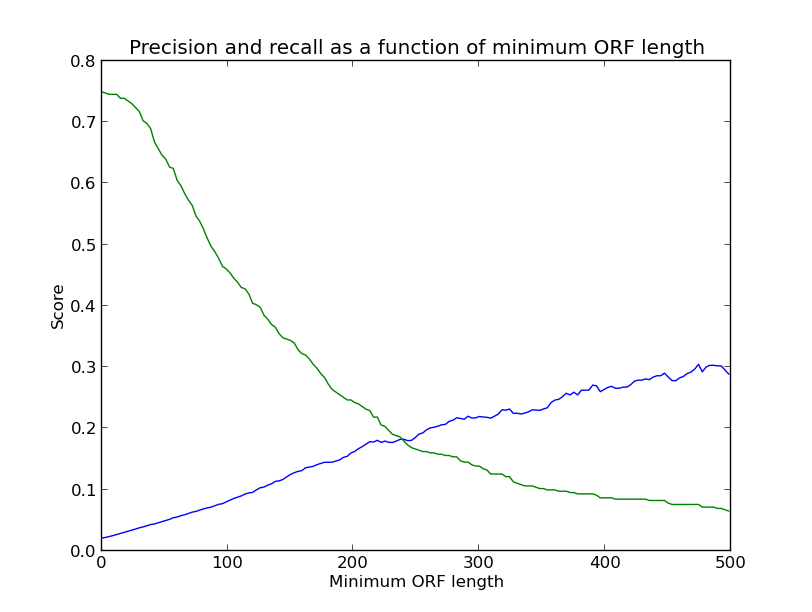
\includegraphics[scale=0.65]{precision-recall.png}
\caption{Precision and recall for Paramecium. Blue line = precision. Green line = recall.}
\label{precrec}
\end{center}
\end{figure}

\subsection{Emiliania huxleyi virus 86}

\subsubsection{Detecting ORFs}
1434 ORFs code for at least 60 amino acids.

\subsubsection{Precision and recall}
In Figure \ref{precrec2} we can see how precision and recall change depending on the minimum ORF length.
\begin{figure}[h!]
\begin{center}
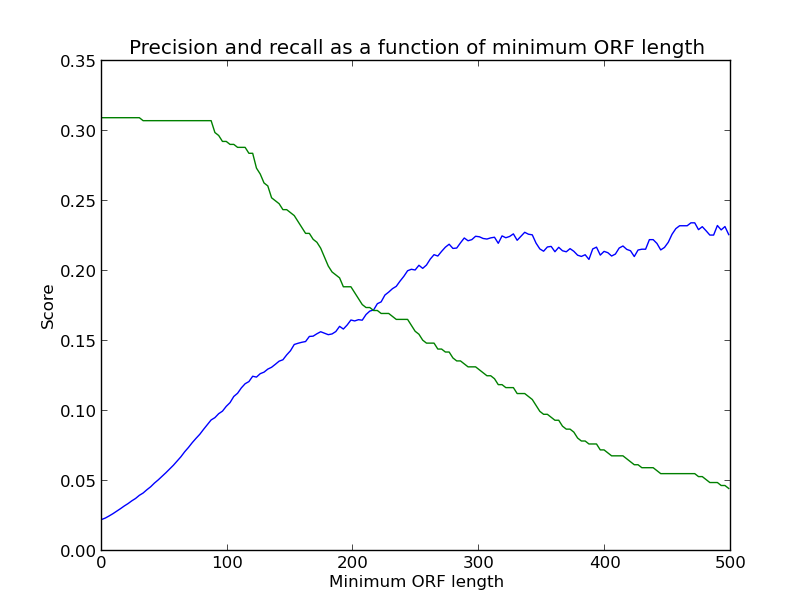
\includegraphics[scale=0.65]{precision-recall2.png}
\caption{Precision and recall in Emiliania huxleyi virus. Blue line = precision. Green line = recall.}
\label{precrec2}
\end{center}
\end{figure}
The scores for precision and recall for 125 codons or more are \textbf{0.6797} and \textbf{0.6653} respectively. 

It seems the \textit{Emiliania huxleyi virus} gave a considerably better score. I am guessing the reason for this is the fact that a virus is a much simpler organism than the \textit{Paramecium}. The virus only has a few functions that need to be executed and the source code for them is not as complex and thus easier to decode.
\section*{Honor Code}

% The following paragraph of your report should be included as is - do % not change it.

My answers to homework are my own work. I did not make solutions or code available to anyone else. I did not engage in any other activities that will dishonestly improve my results or dishonestly improve/hurt the results of others.

\end{document}